\subsection*{Redigering}
Redigering inddeles i en boundary og en tilhørende controller, som det fremgår af \autoref{fig:Redigering}. 

\begin{figure} [H]
\centering
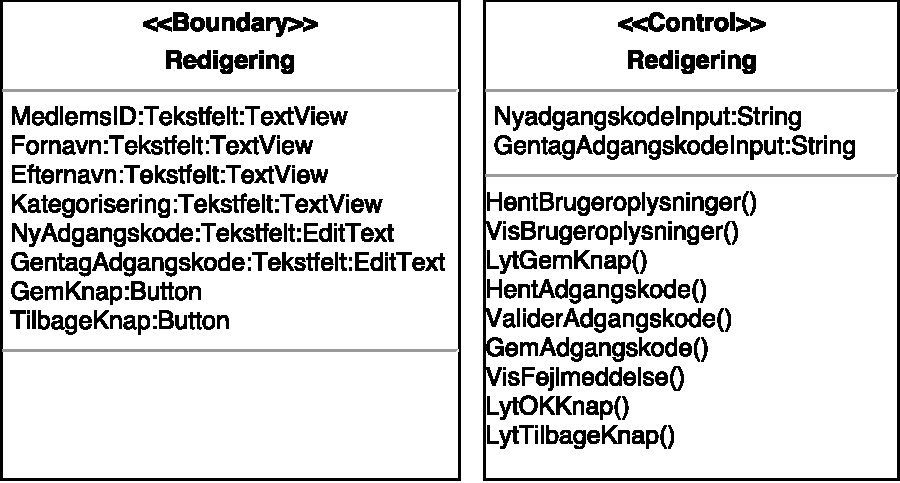
\includegraphics[width=1\textwidth]{figures/MVC/Redigering}
\caption{Designklasser for Redigering. Til venstre fremgår boundary og til højre controller for redigering.}
\label{fig:Redigering}
\end{figure}

\noindent
I grænsefladen for \textit{Redigering} opstilles tekstfelter af typen TextView for medlemsID, navn og kategorisering. Derudover er der tekstfelter, af typen EditText, for ny adgangskode og gentag adgangskode, hvor brugeren kan angive en ny adgangskode. Dertil er der en GemÆndringKnap, af typen Button. GemÆndringKnap indikerer ved tryk, at brugeren ønsker at gemme den nye adgangskode. 
Den tilhørende controller har attributter samt metoder, der omfatter Vis, Lyt, Valider og Send. Valider og Send handler ud fra opstillede inputsparametre. 


Til disse klasser er der opstillet et sekvensdiagram, hvilket fremgår af \autoref{fig:SEKRedigering}.


\begin{figure} [H]
\centering
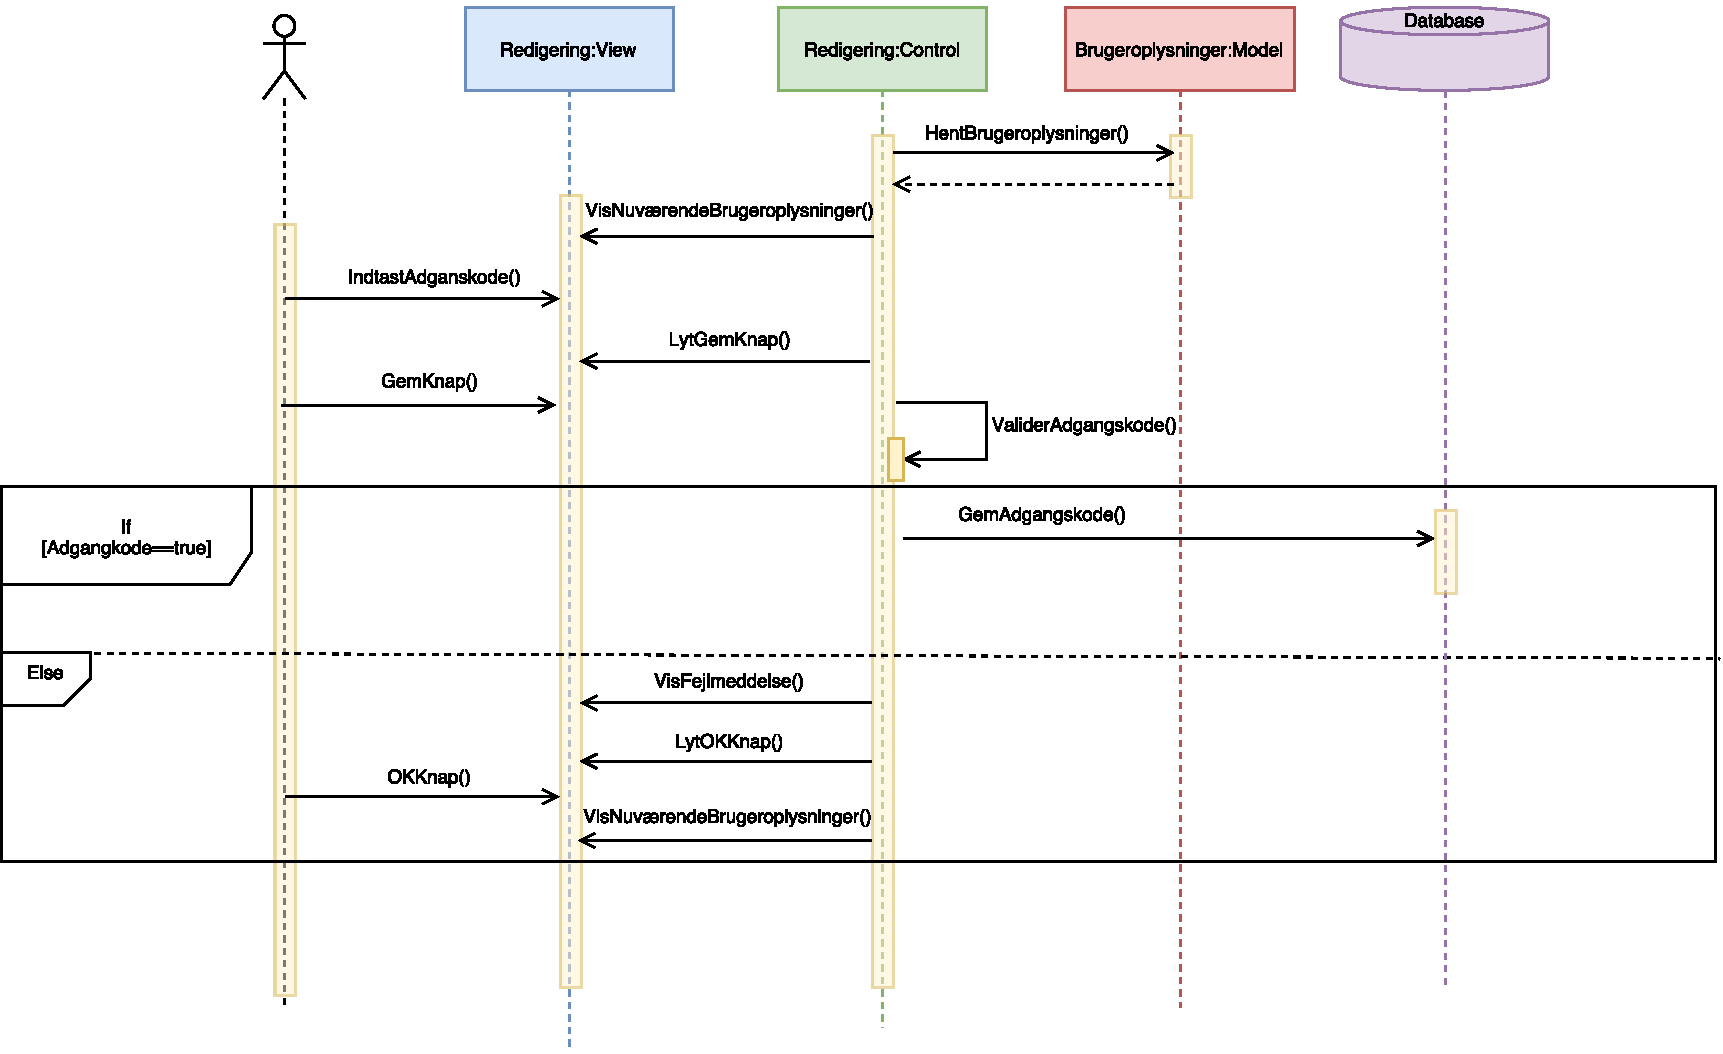
\includegraphics[width=1\textwidth]{figures/Sek/SEKRedigering}
\caption{Sekvensdiagram for redigering.}
\label{fig:SEKRedigering}
\end{figure}

\noindent
\textit{Redigering}-controlleren henter brugeroplysninger, herunder medlemsID, fornavn, efternavn samt kategorisering ved hjælp af get-metoden fra modellen \textit{Brugeroplysninger}. Disse oplysninger vises i grænsefladen for \textit{Redigering}, hvortil brugeren kan se sin information. Fra denne grænseflade er det ligeledes muligt for brugeren at ændre sin adgangskode. Adgangskoden skal indtastes to gange for at sikre, at adgangskoden er identisk. Dertil skal adgangskoden være minimum 10 karakterer lang. Adgangskoden sendes og valideres i \textit{Redigering}-controlleren, hvorefter den sendes til \textit{Database}-controlleren, der gemmer den i \textit{Database}. Overholder adgangskoden ikke de opstillede kriterier, vises en fejlmeddelelse i grænsefladen. Denne forsvinder efter kort tid, hvortil grænsefladen for redigering vises igen. 
